%This is the first real chapter of this thesis. Other chapters can be easily referenced, for example the introduction can be found as Chapter \ref{chapter:introduction}. Sections and/or subsections need to be labeled before one can reference them. See Section \ref{sec:second-section} for an example.

%\section{First Section of the First Chapter}
%Some text in the first section.
%\subsection{First Subsection}
%As well as some text in this subsection.
%\subsubsection{First Subsubsection}
%The Table of Contents only goes 3 layers deep (Chapter - Section - Subsection) so this subsubsection is not seen there.

%\section{Second Section of the First Chapter}\label{sec:second-section}

Projektis kasutatud spordikell on Polar RC3 GPS.

Kellaga on kaasas ka manual, kus on välja toodud kella omadused.\cite{rc3-man}
Konkreetne mudel on toodetud aastal 2013.

\section{Kella riistvara}\label{sec:riistvara}
\begin{figure}[ht]
    \centering
    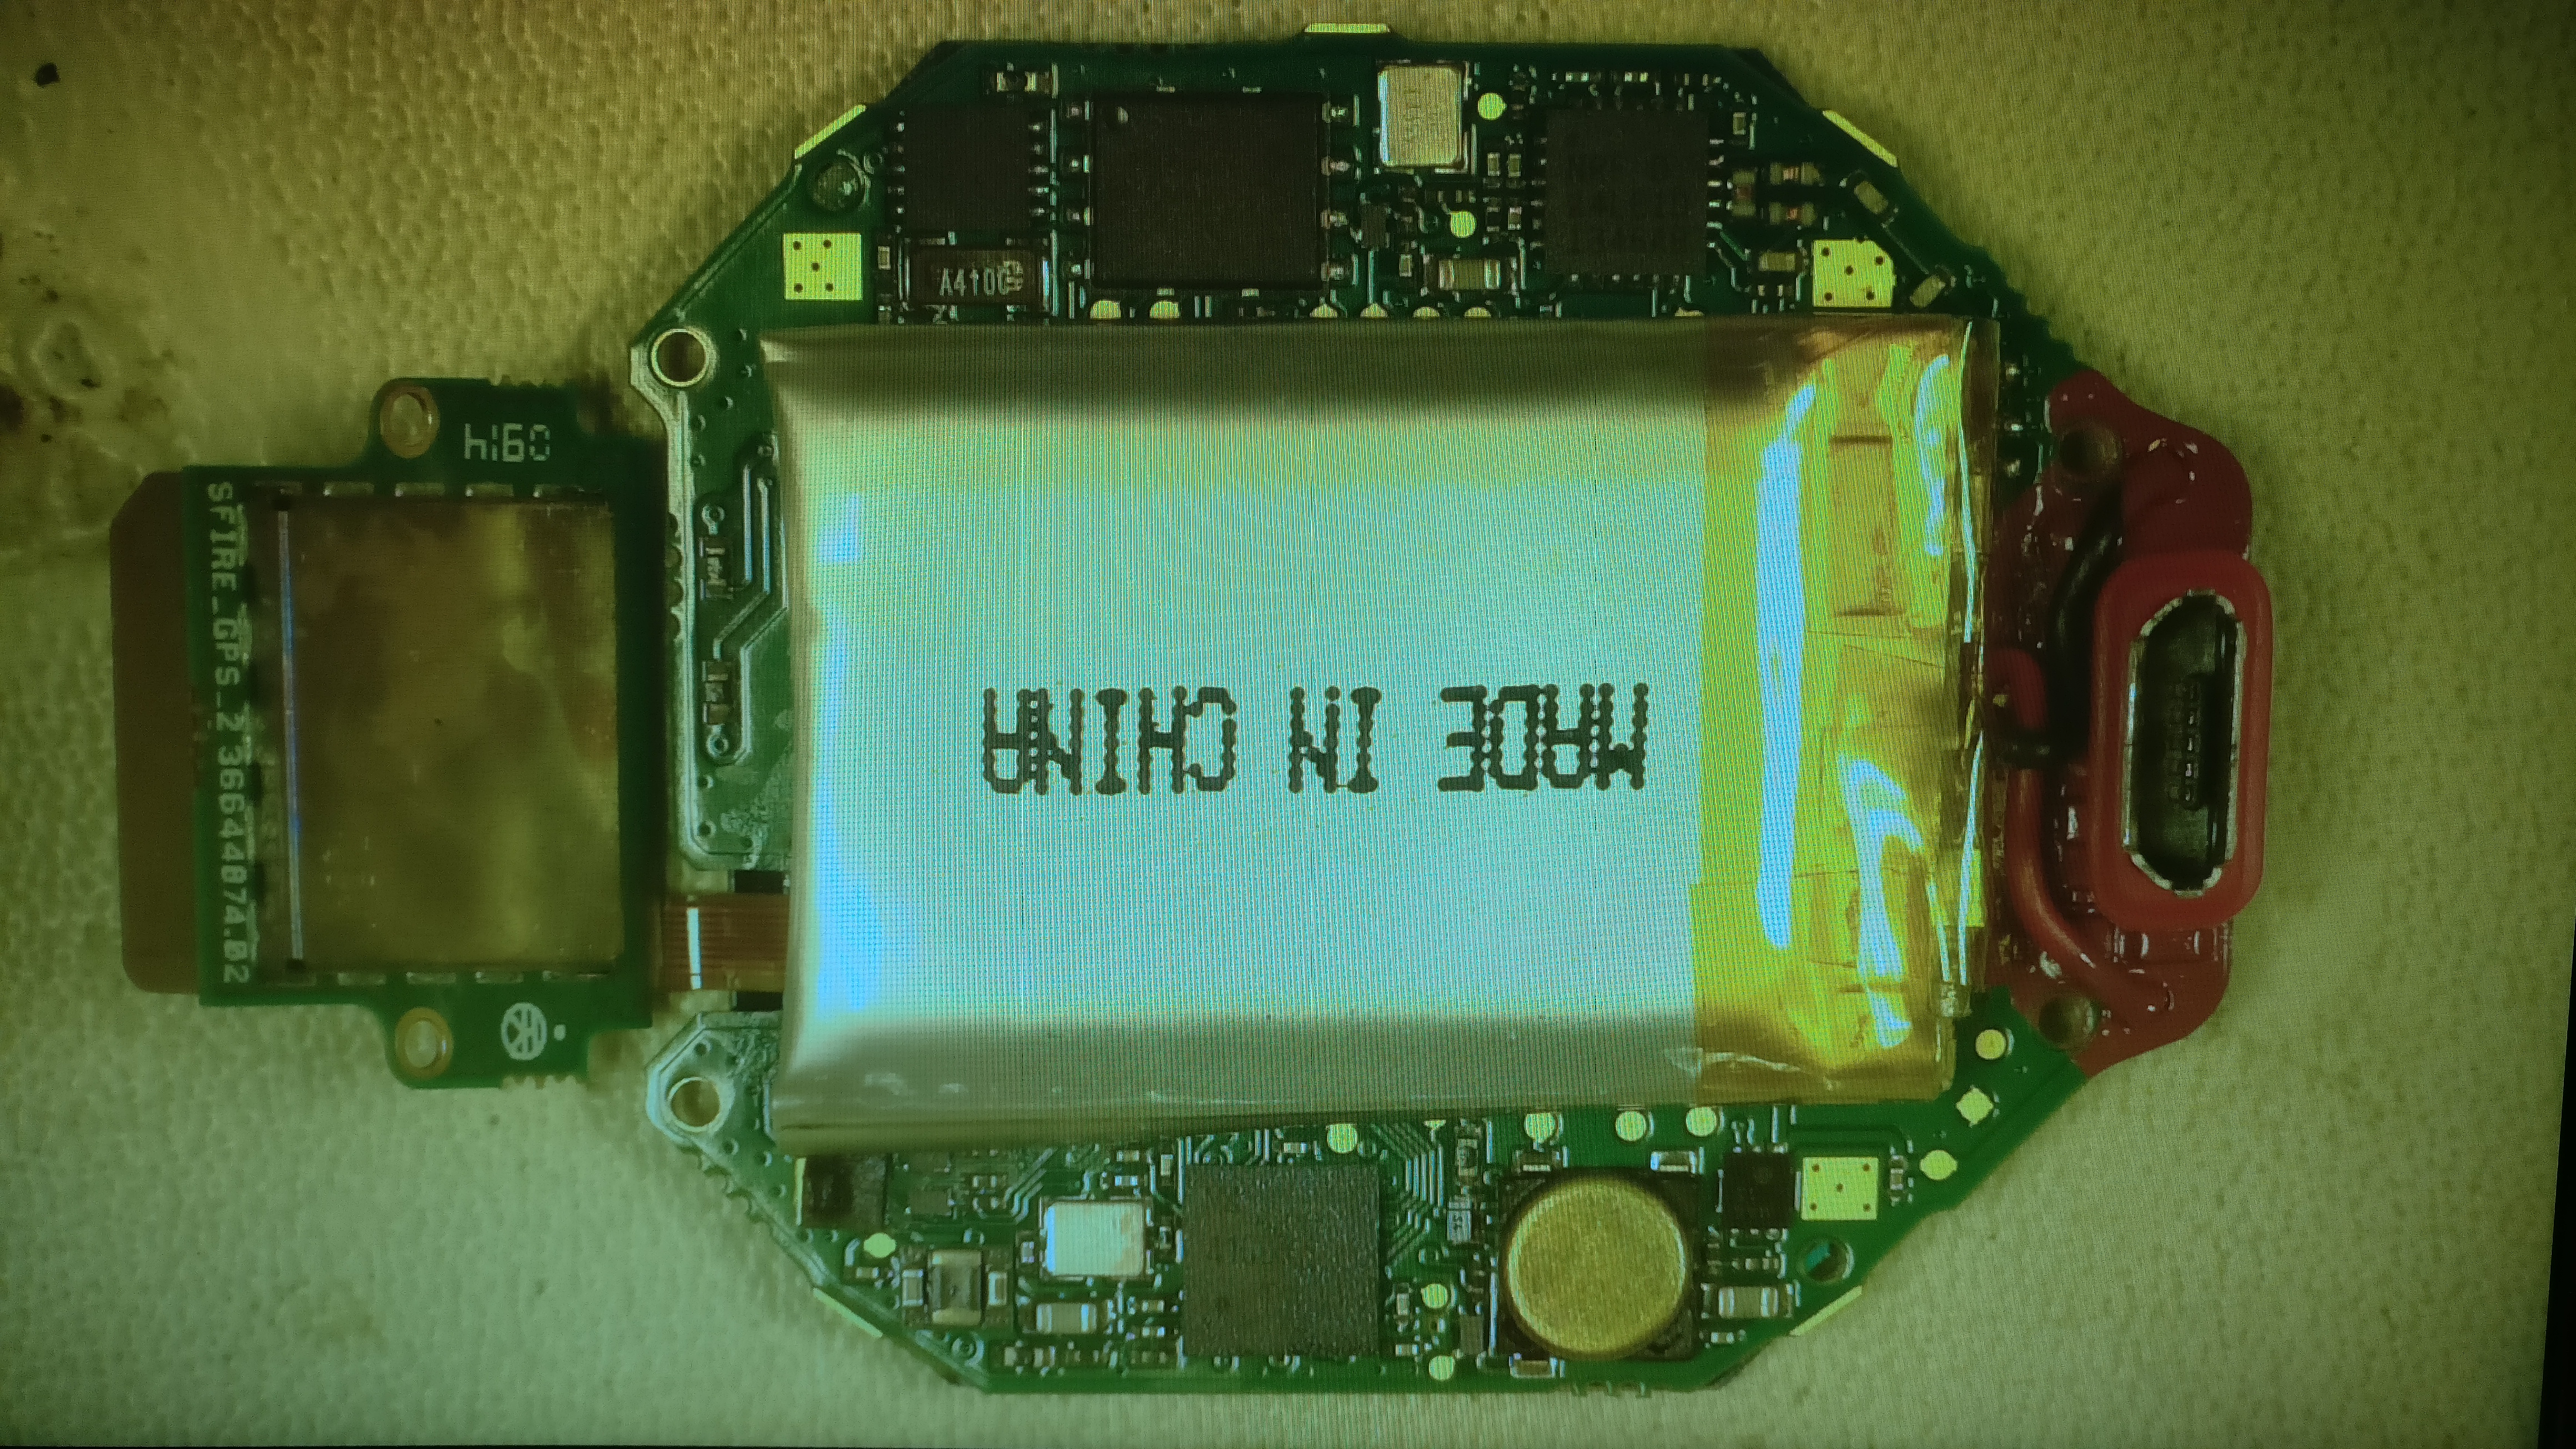
\includegraphics[width=.5\textwidth]{figures/watch.jpg}
    \caption{\textit{Pilt kella emalplaadist}}
    \label{fig:watch}
\end{figure}

Projekti alguses tutvuti ka kella riistvaraga, võttes kell lahti ja uurides selle komponente.
Kuna kella pidi saama ka hiljem kasutada, ei hakatud antud projekti käigus lahti võtma kella komponente, et neid lähemalt uurida.
Kella riistvara kohta avalikku dokumentatsiooni ei leitud ning kella enda emaplaati uurides ka ei olnud lihtne aru saada, millised konkreetsed detailid sellel olid.
Kella uuriti mikroskoobi all ning iga komponendi kohta pandi kirja kõik informatsioon, mis oli võimalik leida.
Hiljem internetist nende komponentide kohta informatsiooni otsimine ei andnud tulemusi, kuna ei olnud võimalik piisavalt täpselt otsida.

\section{Tootjapoolne tarkvara}\label{sec:tootja-soft}
Polari tarkvara, millega sai kellast andmeid tõmmata ja analüüsida, oli Polar WebSync.
Selle tööpõhimõte oli järgnev:
Tuli ühendada kell arvuti külge, seejärel käivitada rakendus.
Andmete kättesaamiseks ja vaatamiseks oli vaja luua kasutajakonto nende veebikeskkonda.
Kui konto oli olemas, tuli logida sisse enda kasutajanime ja parooliga rakendusse, mis seejärel tõmbas andmed kellast pilve, kus neid siis töödeldi ja seejärel sai andmeid veebilehitsejas sisselogituna vaadata. 
Kasutaja masinasse andmeid ei jäetud, nii et neist koopiat teha ei olnud võimalik.
Aasta 2019 lõpus\cite{polar-ws-discontinued} lõpetati toetus ära rakendusele WebSync ja sulgeti ka veebikeskkond polarpersonaltrainer.com, kuna see oli vana ja sooviti keskenduda uue süsteemi toetamisele.
Uus keskkond on tehniliselt erinev vanast, nii et andmete üle toomine ning vana rakenduse kasutamine ei olnud võimalik.
Selle tagajärjel on inimesed, kes kasutavad vana riistvara jäänud ilma võimalusest oma treeningute andmeid analüüsida rohkem, kui kellast iga individuaalse treeningu andmeid vaadates.

Kell suhtleb arvutiga kasutades USB ühendust.

USB standard klassifitseerib ära seadmete klassid. Antud kell klassifitseerub HID seadmeks, mis tähendab seda, et see on seade millega inimesed saavad otseselt kasutada.
HID seadmete jaoks on ette nähtud omaette suhtlusviis, kuidas saab edastada teateid seadmele ja sealt infot kätte.

kirjelda kuidas see suhtlus on et koigepealt avad jne 

siis kuidas see muu osa seal on et ei taha seda surnuks pommitada

mis asjad on endpointid jne

